\documentclass[]{book}
\usepackage{lmodern}
\usepackage{amssymb,amsmath}
\usepackage{ifxetex,ifluatex}
\usepackage{fixltx2e} % provides \textsubscript
\ifnum 0\ifxetex 1\fi\ifluatex 1\fi=0 % if pdftex
  \usepackage[T1]{fontenc}
  \usepackage[utf8]{inputenc}
\else % if luatex or xelatex
  \ifxetex
    \usepackage{mathspec}
  \else
    \usepackage{fontspec}
  \fi
  \defaultfontfeatures{Ligatures=TeX,Scale=MatchLowercase}
\fi
% use upquote if available, for straight quotes in verbatim environments
\IfFileExists{upquote.sty}{\usepackage{upquote}}{}
% use microtype if available
\IfFileExists{microtype.sty}{%
\usepackage{microtype}
\UseMicrotypeSet[protrusion]{basicmath} % disable protrusion for tt fonts
}{}
\usepackage[margin=1in]{geometry}
\usepackage{hyperref}
\hypersetup{unicode=true,
            pdftitle={Sleep quality analysis},
            pdfauthor={Arturo Laflor},
            pdfborder={0 0 0},
            breaklinks=true}
\urlstyle{same}  % don't use monospace font for urls
\usepackage{natbib}
\bibliographystyle{apalike}
\usepackage{longtable,booktabs}
\usepackage{graphicx,grffile}
\makeatletter
\def\maxwidth{\ifdim\Gin@nat@width>\linewidth\linewidth\else\Gin@nat@width\fi}
\def\maxheight{\ifdim\Gin@nat@height>\textheight\textheight\else\Gin@nat@height\fi}
\makeatother
% Scale images if necessary, so that they will not overflow the page
% margins by default, and it is still possible to overwrite the defaults
% using explicit options in \includegraphics[width, height, ...]{}
\setkeys{Gin}{width=\maxwidth,height=\maxheight,keepaspectratio}
\IfFileExists{parskip.sty}{%
\usepackage{parskip}
}{% else
\setlength{\parindent}{0pt}
\setlength{\parskip}{6pt plus 2pt minus 1pt}
}
\setlength{\emergencystretch}{3em}  % prevent overfull lines
\providecommand{\tightlist}{%
  \setlength{\itemsep}{0pt}\setlength{\parskip}{0pt}}
\setcounter{secnumdepth}{5}
% Redefines (sub)paragraphs to behave more like sections
\ifx\paragraph\undefined\else
\let\oldparagraph\paragraph
\renewcommand{\paragraph}[1]{\oldparagraph{#1}\mbox{}}
\fi
\ifx\subparagraph\undefined\else
\let\oldsubparagraph\subparagraph
\renewcommand{\subparagraph}[1]{\oldsubparagraph{#1}\mbox{}}
\fi

%%% Use protect on footnotes to avoid problems with footnotes in titles
\let\rmarkdownfootnote\footnote%
\def\footnote{\protect\rmarkdownfootnote}

%%% Change title format to be more compact
\usepackage{titling}

% Create subtitle command for use in maketitle
\newcommand{\subtitle}[1]{
  \posttitle{
    \begin{center}\large#1\end{center}
    }
}

\setlength{\droptitle}{-2em}
  \title{Sleep quality analysis}
  \pretitle{\vspace{\droptitle}\centering\huge}
  \posttitle{\par}
  \author{Arturo Laflor}
  \preauthor{\centering\large\emph}
  \postauthor{\par}
  \predate{\centering\large\emph}
  \postdate{\par}
  \date{2017-05-03}

\usepackage{booktabs}
\usepackage{amsthm}
\usepackage{multirow}
\usepackage{multicol}
\usepackage{float}
\usepackage{tabularx}
\makeatletter
\def\thm@space@setup{%
  \thm@preskip=8pt plus 2pt minus 4pt
  \thm@postskip=\thm@preskip
}
\makeatother

\begin{document}
\maketitle

{
\setcounter{tocdepth}{1}
\tableofcontents
}
\chapter{Prerequisites}\label{prerequisites}

\chapter{Introduction}\label{intro}

\hypertarget{data-adquisition}{\chapter{\texorpdfstring{\protect\hyperlink{data-adquisition}{Data
adquisition}}{Data adquisition}}\label{data-adquisition}}

\chapter{\texorpdfstring{\protect\hyperlink{data-preprocess}{Data
pre-process}}{Data pre-process}}\label{data-pre-process}

\hypertarget{feature-selection}{\chapter{\texorpdfstring{\protect\hyperlink{feature-selection}{Feature
selection}}{Feature selection}}\label{feature-selection}}

\chapter{\texorpdfstring{\protect\hyperlink{efficiency-evaluation}{Evaluation
of
Efficiency}}{Evaluation of Efficiency}}\label{evaluation-of-efficiency}

One of the steps in the development of the investigation project,
includes the selection of a technique to train a predictive model on
supervised automated learning. We did a review of the literature and we
select three techniques under certain criterion based in the nature of
the problem. The purpose is train the model with the available data and
select the one given the best prediction. So, at the same time that the
evaluation of efficience of the selected factors was performed, the
selection of the technique that will be used for the final training was
done. The three techniques that meet the inclusion criteria, were:
artificial neural networks, vector supported machines And logistic
regression with regularization. As in feature selection, a Shiny
application was developed to process the data and compare the outcomes
for these three algorithms, training a model with total of the records
and only the four features selected in the feature selection process as
was explained in Section \ref{feature-selection}.

The evaluation was performed by the cross validation technique using an
iteration process of training, validation, analysis and refinement as
the figure \ref{fig:cross-validation-process} shows. In this process a
sixty percent of the data was used to train the model, when training
conclude, the cross validation is performed through the prediction of
the target variable in the cross validation set, containing a twenty
percent of the main dataset. The analysis is done at that time and
depending on the results, the parameters are adjusted to make a new
iteration or reach the stop point. If the stop point was reached, the
model is proved in the test set to obtain the final efficience of the
model.

\begin{figure}[H]

{\centering 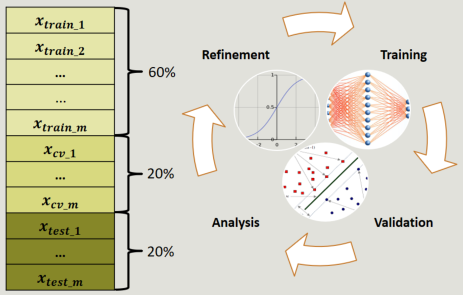
\includegraphics[width=0.8\linewidth]{images/cross-validation-process} 

}

\caption{Cross Validation Process}\label{fig:cross-validation-process}
\end{figure}

\hypertarget{neural-networks-results}{\section{\texorpdfstring{\protect\hyperlink{neural-networks-results}{Neural
Networks
Results}}{Neural Networks Results}}\label{neural-networks-results}}

Two neural networks were trained and validated by cross validation
process, both estructures with a hidden layer. The first neural network
had three neurons in the hidden layer and the second four neurons. The
Fig. \ref{fig:nn-four-neurons} shows the structure of the neural network
with four neurons in the input layer, one neuron for each factor
selected in the feature selection process. The second layer is the
hidden layer with four neurons and the last layer contains one neuron
for the result (good sleep quality/bad sleep quality). Additionaly it is
possible to observe the two activation neurons in the top of the figure.

\begin{figure}[H]

{\centering 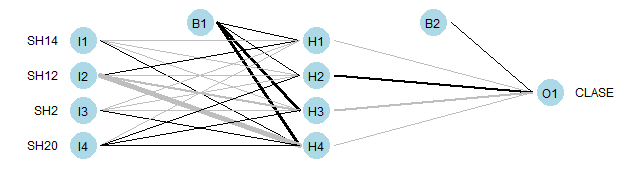
\includegraphics[width=0.8\linewidth]{images/nn-four-neurons} 

}

\caption{Structure of neural network with four neurons in the hidden layer}\label{fig:nn-four-neurons}
\end{figure}

The results for the two neural networks and the appropriate comparison
are presented in the Fig. \ref{fig:results-of-the-3-4-nn}. The network
with better efficiency of two networks is the network with four neurons.
The table describes that in the three sets, the behavior was superior in
terms of efficiency, while the plot represents the error per each set
with three and four neurons. CClearly, the lines decrease in favor of
the training and validation with four neurons, where the error of the
prediction is smaller.

\begin{figure}[H]

{\centering 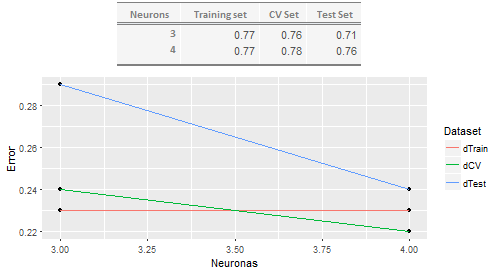
\includegraphics[width=0.8\linewidth]{images/results-of-the-3-4-nn} 

}

\caption{Comparison of the results for the two trained neural networks}\label{fig:results-of-the-3-4-nn}
\end{figure}

\chapter{Applications}\label{applications}

\chapter{Placeholder}\label{placeholder}

\chapter{Final Words}\label{final-words}

\bibliography{packages,book}


\end{document}
